\documentclass[25pt, a0paper, landscape]{tikzposter}

% ============================================================
% Packages
% ============================================================
\usepackage[T1]{fontenc}
\usepackage[sfdefault]{FiraSans}
\usepackage{lmodern}
\usepackage{graphicx}
\usepackage{enumitem}

% Remove tikzposter watermark
\tikzposterlatexaffectionproofoff

% Define VeryHuge if not available in this tikzposter version
\makeatletter
\@ifundefined{VeryHuge}{%
  \newcommand{\VeryHuge}{\fontsize{80}{96}\selectfont}%
}{}
\makeatother

% ============================================================
% Color Theme — RoCam Red / Black
% ============================================================
\definecolorstyle{RoCamStyle}{
  \definecolor{colorOne}{RGB}{30, 30, 30}       % dark (headers)
  \definecolor{colorTwo}{RGB}{220, 38, 38}      % RoCam red
  \definecolor{colorThree}{RGB}{245, 245, 245}  % light gray
}{
  \colorlet{backgroundcolor}{white}
  \colorlet{framecolor}{white}
  % title bar
  \colorlet{titlefgcolor}{white}
  \colorlet{titlebgcolor}{colorOne}
  % blocks
  \colorlet{blocktitlebgcolor}{colorOne}
  \colorlet{blocktitlefgcolor}{white}
  \colorlet{blockbodybgcolor}{white}
  \colorlet{blockbodyfgcolor}{black}
  % inner blocks
  \colorlet{innerblocktitlebgcolor}{colorTwo}
  \colorlet{innerblocktitlefgcolor}{white}
  \colorlet{innerblockbodybgcolor}{colorThree}
  \colorlet{innerblockbodyfgcolor}{black}
}

\usetheme{Default}
\usecolorstyle{RoCamStyle}
\useblockstyle{Default}
\usetitlestyle{Filled}
\makeatletter
\setlength{\TP@blockverticalspace}{8mm}
\makeatother

% Consistent image card for poster visuals
\newcommand{\posterimg}[3][]{%
  \begin{minipage}[t]{\linewidth}
    \centering
    \setlength{\fboxsep}{0pt}%
    \fcolorbox{colorOne!40}{white}{\includegraphics[#1]{#2}}\\[0.12em]
    {\footnotesize\bfseries #3}
  \end{minipage}%
}

% Section header colors
\definecolor{motivationColor}{RGB}{146, 32, 57}
\definecolor{architectureColor}{RGB}{0, 102, 128}
\definecolor{toolsColor}{RGB}{168, 96, 24}
\definecolor{featuresColor}{RGB}{34, 108, 76}
\definecolor{visionColor}{RGB}{58, 78, 146}
\definecolor{teamColor}{RGB}{105, 74, 42}

\newcommand{\sectionblock}[3]{%
  {%
    \colorlet{blocktitlebgcolor}{#1}%
    \colorlet{blocktitlefgcolor}{white}%
    \block{#2}{#3}%
  }%
}

% ============================================================
% Title — three-part header: McMaster | Logo+Title | Department
% ============================================================
\title{\mbox{}}
\author{}
\institute{}

% --- Override title colors to Grey Background and Black Text ---
\colorlet{titlebgcolor}{gray!20}
\colorlet{titlefgcolor}{black}

\makeatletter
\settitle{
  \parbox{\linewidth}{%
    \color{titlefgcolor}%
    \begin{minipage}[c]{0.20\linewidth}
      \centering
      \makebox[\linewidth][c]{%
        \makebox[0pt][c]{%
          \smash{%
            \raisebox{0.15cm}[0pt][0pt]{%
                \begin{tikzpicture}
                % Removed opacity=0.42 and increased height to 10.0cm
                \node[inner sep=0pt, outer sep=0pt]
                    {
\includegraphics[height=5.0cm]{libs/McMaster_University_logo.svg.png}};
                \end{tikzpicture}
            }%
          }%
        }%
        \parbox[c]{0.92\linewidth}{\centering {\Large\bfseries McMaster University}\\[0.15em]{\Large Engineering}}
      }
    \end{minipage}%
    \hfill
    \begin{minipage}[c]{0.52\linewidth}
      \centering
      \includegraphics[height=7cm]{../../../assets/logo/red.png}\\[0.3em]
      {\huge High Performance Vision-Guided Rocket Tracker}
    \end{minipage}%
    \hfill
    \begin{minipage}[c]{0.22\linewidth}
      \raggedleft
      {\LARGE\bfseries Capstone Project}\\[0.3em]
      {\Large Department of\\Computing and Software\\[0.2em]}
    \end{minipage}%
  }%
}
\makeatother

% ============================================================
\begin{document}
\maketitle

\begin{columns}

% ============================================================
%  LEFT COLUMN
% ============================================================
\column{0.48}

% --- Motivation ---
\sectionblock{motivationColor}{Motivation}{
  \textbf{The Problem:} Model rockets accelerate to extreme speeds within fractions of a second, making manual camera tracking virtually impossible. Existing commercial tracking systems are cost-prohibitive and lack the precision required for small, fast-moving targets. Consequently, rocketry teams lose critical visual data for mid-flight events like staging and parachute tangling.

  \vspace{0.5em}

  \textbf{The Solution:} RoCam bridges this gap with an \textbf{autonomous, vision-guided tracking system}. By locking onto the rocket in real time, it actively commands a two-axis gimbal to deliver smooth \textbf{1080p video at 60\,fps}. 

  \vspace{0.5em}

  \centering
  \posterimg[
    width=0.96\linewidth,
    keepaspectratio
  ]{libs/section_1.png}{RoCam Launch and Tracking Operations}
}

% --- System Architecture ---
\sectionblock{architectureColor}{System Architecture}{
  % --- Left Side: Diagram ---
  \begin{minipage}[c]{0.58\linewidth}
    \centering
    \posterimg[
      width=\linewidth,
      clip
    ]{../../../img/pipeline.png}{Real-Time Vision and Control Pipeline}
  \end{minipage}% <--- Crucial % to prevent Overfull \hbox
  \hfill
  % --- Right Side: Text ---
  \begin{minipage}[c]{0.40\linewidth}
    \small
    \noindent\textbf{Edge Compute \& Hardware.} The implemented architecture follows a distributed multi-process edge-compute design on an NVIDIA Jetson. To ensure high reliability, CPU/GPU-heavy perception workloads are isolated from control and operator services via Inter-Process Communication (IPC). This strict fault isolation preserves deterministic command flow and API stability even if the vision pipeline encounters transient errors during launch-dynamic conditions.

    \vspace{0.6em}
    \noindent\textbf{Vision Pipeline.} Image acquisition utilizes a GStreamer capture graph configured for 1920$\times$1080 at 60\,fps, feeding NVIDIA DeepStream for GPU-accelerated preprocessing. Detection relies on a YOLO network optimized with TensorRT, yielding low-latency normalized bounding boxes. A decoupled Live Video process parallelizes OSD telemetry overlay and HDMI output to guarantee continuous situational awareness without blocking inference.

    \vspace{0.6em}
    \noindent\textbf{Kinematic Control.} The tracking module calculates image-plane target error (targeting frame center $cx=0.5, cy=0.5$) to generate proportional 2-axis gimbal actuation commands. These commands pass through a validated, state-gated pathway—enforcing rate limits and safety bounds—before transmission to an STM32 microcontroller via UART, ensuring deterministic, closed-loop responsiveness throughout boost and coast regimes.

    \vspace{0.6em}
    \noindent\textbf{Backend \& State Management.} System orchestration is governed by a centralized State Machine (Disarmed, Armed, Tracking, Recording) that prevents invalid mode combinations and enforces hardware safety. A Flask-based API Gateway exposes a REST interface for offline-first LAN operation, managing mode transitions, asynchronous recording/transcoding workflows, and streaming SSE telemetry for live state and control-stream observability.
  \end{minipage}
}

% --- Tools & Technologies ---
\sectionblock{toolsColor}{Tools \& Technologies}{
  \vspace{-0.6em} % Pulls the image up tightly against the title
  \centering
  
\includegraphics[width=0.85\linewidth, keepaspectratio]{libs/tools.png}
  \vspace{-0.4em} % Shaves off extra white space at the bottom of the block
}

% ============================================================
%  RIGHT COLUMN
% ============================================================
\column{0.48}

\sectionblock{featuresColor}{Software \& Hardware Features}{
  \begin{minipage}[t]{0.48\linewidth}
    \vspace{0pt}
    \centering
    % Images now share identical width, height, and ratio constraints
    
\includegraphics[width=0.58\linewidth, height=4.5cm, keepaspectratio]{libs/team_placeholder.png}\\[0.3em]
    {\normalsize\bfseries Web-Based Operator Interface}\\[0.45em]
    \small
    \raggedright
    \begin{itemize}[leftmargin=1.1em, itemsep=0.1em, topsep=0pt, parsep=0pt]
        \item \textbf{Real-Time Gimbal Control:} Low-latency control path between the operator interface and an STM32-based pan-tilt gimbal controller for immediate physical camera motion.
        \item \textbf{Manual Positioning:} In \textbf{idle} mode, the operator can manually pan and tilt the camera in real time to align the view with the launch rail or expected ascent corridor.
        \item \textbf{Remote Operation:} Core control actions are available through a browser over a local network, allowing safe stand-off operation without internet access.
        \item \textbf{System-State Awareness:} Clear visual feedback on the current state (\textbf{idle}, \textbf{armed}, \textbf{tracking}) to quickly verify readiness during time-critical procedures.
        \item \textbf{Safe Override:} Operator can immediately stop automated motion and return to a safe \textbf{idle} state for fault recovery or unexpected target behavior.
    \end{itemize}
  \end{minipage}%
  \hfill
  \begin{minipage}[t]{0.48\linewidth}
    \vspace{0pt}
    \centering
    % Images now share identical width, height, and ratio constraints
    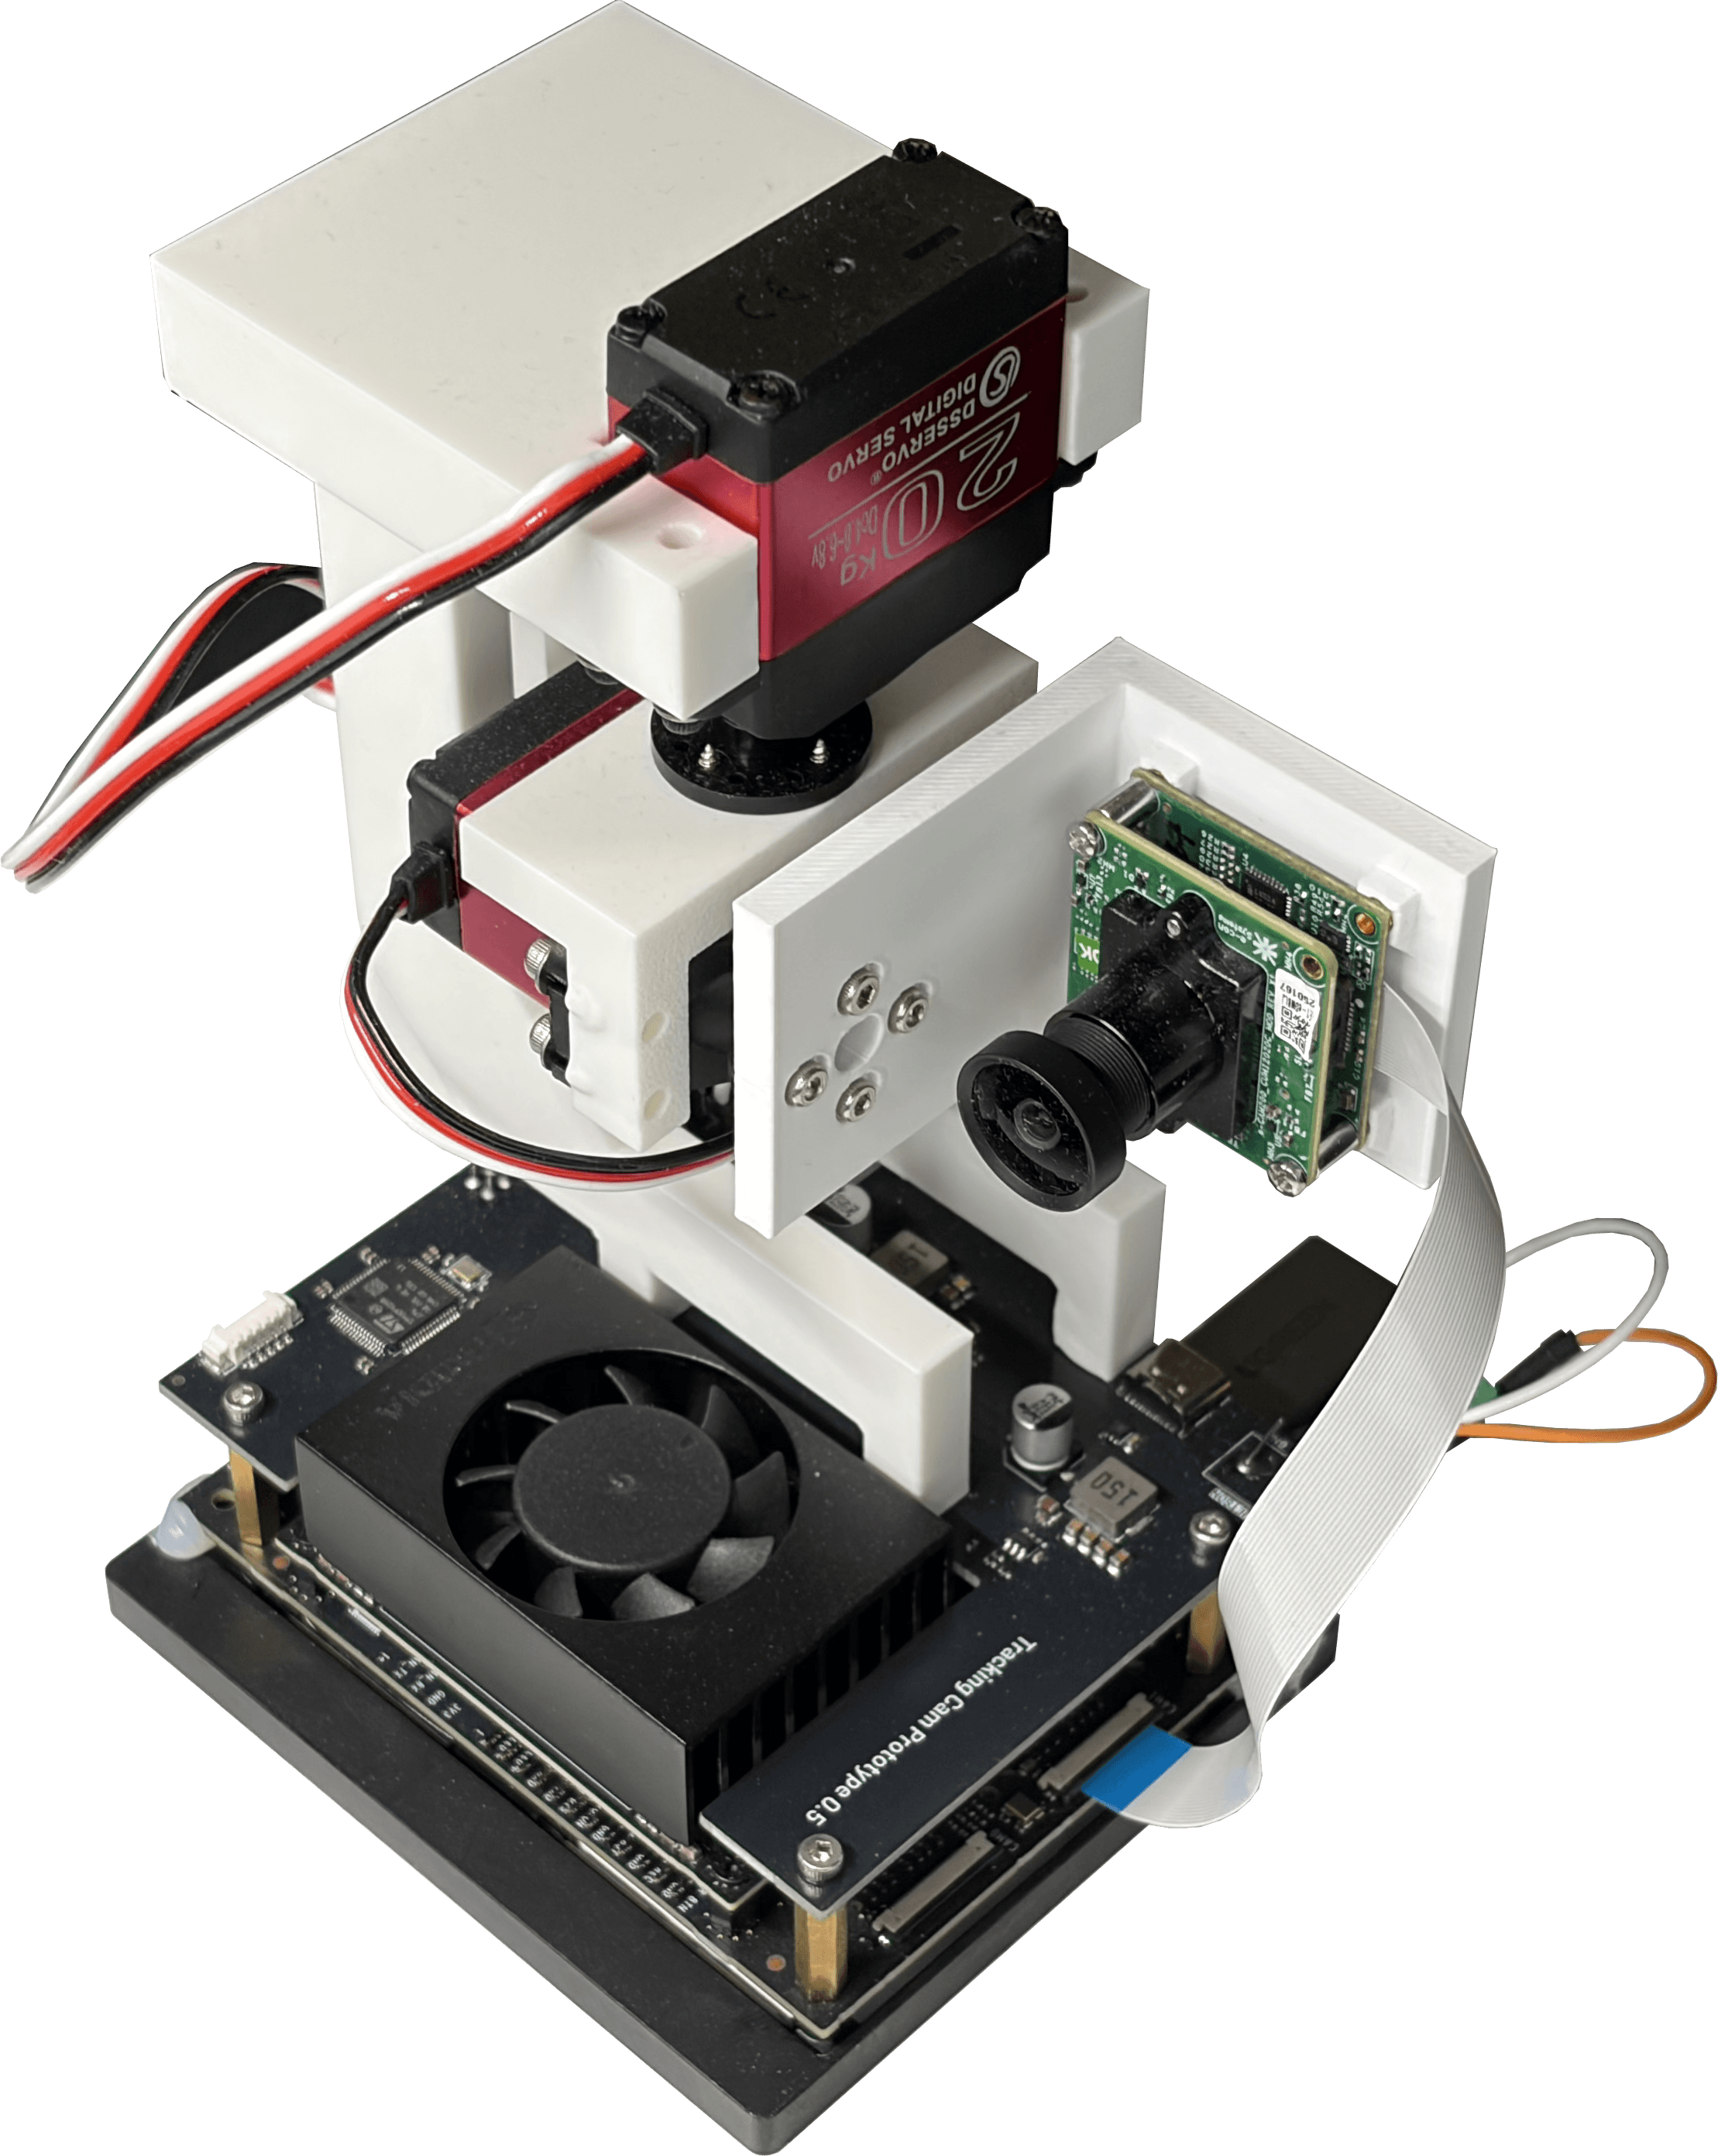
\includegraphics[width=0.58\linewidth, height=4.5cm, keepaspectratio]{libs/prototype.png}\\[0.3em]
    {\normalsize\bfseries Two-Axis Gimbal Prototype}\\[0.45em]
    \small
    \raggedright
    \begin{itemize}[leftmargin=1.1em, itemsep=0.1em, topsep=0pt, parsep=0pt]
        \item \textbf{Autonomous Vision Tracking:} Once \textbf{armed}, RoCam continuously processes the live feed to detect the rocket as a fast-moving target under realistic conditions.
        \item \textbf{Automatic State Transition:} Automatically transitions from \textbf{armed} to \textbf{tracking} upon valid detection, reducing reaction delay during critical flight phases.
        \item \textbf{Closed-Loop Target Following:} Vision pipeline detections are converted into continuous pan and tilt corrections to keep the rocket centered throughout the flight.
        \item \textbf{Robustness in Challenging Conditions:} Effective against common launch disturbances such as smoke plumes, glare, motion blur, and rapid angular movement.
        \item \textbf{Short-Term Re-Acquisition:} Attempts to re-acquire the target if briefly lost, improving tracking continuity and preserving flight footage without manual intervention.
    \end{itemize}
  \end{minipage}
}

% ============================================================
%  Machine Learning Section
% ============================================================
\sectionblock{visionColor}{Computer Vision \& Machine Learning}{
  \begin{minipage}[t]{0.28\linewidth}
    \vspace{0pt}
    \centering
    \posterimg[
      width=0.95\linewidth,
      keepaspectratio
    ]{libs/results_train.png}{YOLO26s-P2 Training Performance}
  \end{minipage}%
  \hfill
  \begin{minipage}[t]{0.68\linewidth}
    \vspace{0pt}
    \small
    \raggedright % <--- Added to fix Underfull \hbox warnings
    \begin{itemize}[leftmargin=1.1em, itemsep=0.2em]
    \item \textbf{Architecture Upgrade (YOLO26s-P2):} Added a \textbf{stride-4 detection head} to quadruple the spatial resolution of the finest feature map, ensuring sensitivity to micro-targets as small as $10{\times}10$ pixels.
    
    \item \textbf{Data Engineering \& Hard Negative Mining:} Engineered an automated pipeline to inject \textbf{4,000 pure background COCO images} ($\sim$25\% of the dataset) with empty labels, forcing a harder decision boundary to suppress false positives.
    
    \item \textbf{Custom Degradation Pipeline:} Integrated a DDP-compatible Albumentations pipeline to simulate real-world flight conditions, including motion blur, sensor noise, dynamic range shifts, and compression artifacts.
    
    \item \textbf{Curriculum Augmentation Strategy:} Implemented a progressive reduction strategy across training stages—shifting from heavy augmentation (exploration) to minimal perturbation (exploitation). 
    
    \item \textbf{Failure Analysis \& Debugging:} Diagnosed a critical "Mosaic Starvation" failure where early stopping preempted the \texttt{close\_mosaic} phase, trapping the model on $\frac{1}{4}$-scale downscaled images and crashing mAP$_{50-95}$ to 0.614.
    
    \item \textbf{Close-Mosaic Fine-Tuning:} Engineered a dedicated recovery stage (mosaic=0.0) to expose the model to full-resolution $960{\times}544$ frames, rescuing the pipeline and triggering a massive $+17.3\%$ metric jump.
        
    \item \textbf{HPC Distributed Training:} Orchestrated the complete four-stage training pipeline on a \textbf{4$\times$NVIDIA H100 PCIe (81\,GB)} cluster using Distributed Data Parallel (DDP) and mixed precision.
    \end{itemize}
    \vspace{0.5em}
    \textbf{Final Deployment Metrics:} {\Large \textcolor{colorTwo}{\textbf{mAP$_{50} = 0.958$}; \textbf{mAP$_{50-95} = 0.750$}}}
  \end{minipage}
}

% --- Team Section ---
\sectionblock{teamColor}{Our Team}{
  \begin{minipage}[t]{0.28\linewidth}
    
    % --- COLOR CHANGE ADDED HERE ---
    \colorlet{innerblocktitlebgcolor}{green!40!black} 
    \colorlet{innerblocktitlefgcolor}{white}          
    % -------------------------------

    \innerblock{Development Team}{
      \small\sffamily 
      % Height aggressively reduced to 3.2cm
      \begin{minipage}[t][3.2cm][c]{\linewidth} 
        \centering
        % Image height reduced to 1.3cm, spacing tightened
        
\includegraphics[width=0.85\linewidth, height=1.3cm, keepaspectratio]{libs/team_rocam.png}\\[0.2em]
        Zifan Si \quad Jianqing Liu \\[0.05em]
        Mike Chen \quad Xiaotian Lou
      \end{minipage}
    }
  \end{minipage}%
  \hfill
  \begin{minipage}[t]{0.28\linewidth}
    \innerblock{Launch Team}{
      \small\sffamily
      \begin{minipage}[t][3.2cm][c]{\linewidth}
        \centering
        
\includegraphics[width=0.85\linewidth, height=1.5cm, keepaspectratio]{libs/team_rocketry.png}\\[0.2em]
        McMaster Rocketry Team
      \end{minipage}
    }
  \end{minipage}%
  \hfill
  \begin{minipage}[t]{0.28\linewidth}
    
    % --- COLOR CHANGE ADDED HERE ---
    \colorlet{innerblocktitlebgcolor}{blue!80!black} 
    \colorlet{innerblocktitlefgcolor}{white}         
    % -------------------------------

    \innerblock{Advisory Team}{
      \small\sffamily
      \begin{minipage}[t][3.2cm][c]{\linewidth}
        \centering
        Dr.\ Shahin Sirouspour \quad Dr.\ Spencer Smith \\[0.05em] 
        Tanya Djavaherpour\\[0.2em]
        
\includegraphics[width=0.85\linewidth, height=1.3cm, keepaspectratio]{libs/team_cas.png}
      \end{minipage}
    }
  \end{minipage}
}
\end{columns}
\end{document}
